\chapter{INTRODUÇÃO}\label{CAP:introducao}
%\thispagestyle{empty}
O último levantamento feito pelo IBGE (Instituto Brasileiro de Geografia e Estatísticas) no Brasil indica que existem cerca de 45,6 milhões de pessoas com deficiência \citeonline{IBGE:2010}, representando 23,9\% da população brasileira; deste total 7\% apresentam deficiências motoras que englobam desde restrições suaves até outras severas, estas esferas de indivíduos com condições singulares equivalem a cerca de 3,192 milhões de pessoas no Brasil em 2010. Apesar deste valor expressivo as tecnologias que poderiam possibilitar uma ampliação das habilidades desses indivíduos são pouco exploradas.

O ininterrupto desenvolvimento de novos sistemas, softwares e hardwares concebem uma ampla evolução nas estruturas sociais, corporativas e acadêmicas, porém existem áreas ainda pouco exploradas. Entre elas, é possível destacar a concepção de sistemas baseados em Tecnologia Assistiva (TA).

O conceito de TA, apesar de recente, pode ser definido como o conjunto de sistemas, tecnologias e inovações que permitem aumentar as habilidades funcionais de uma pessoa com algum tipo de deficiência e, desta forma, possibilitar sua inclusão. Segundo \citeonline{Bersch}, o objetivo de TA é proporcionar à pessoa com deficiência maior independência, qualidade de vida e inclusão social, através da ampliação de sua comunicação, mobilidade, controle de ambiente, habilidades de aprendizado, trabalho e integração com a família, amigos e sociedade.

O grande desafio de criar as condições necessárias à acessibilidade das Tecnologias da Informação e Comunicação (TICs) por pessoas com deficiência, transformando a interação desses usuários o mais simples possível, é presente dentro da área de Interação Humano Computador (IHC). É evidente que as características humanas e os estilos de interação são fatores determinantes no modo como é feita a interação com as TICs através das tecnologias.

Tendo em vista os fatores já citados, as motivações pessoas e éticas e as áreas de interesse como TA, Visão Computacional (VC), Inteligência Artificial (IA) e Processamento Digital de Imagens (PDI) manifestou-se a inspiração de desenvolver uma Tecnologia capaz de permitir o uso de um Computador comum por pessoas com algum tipo de deficiência físico-motora por meio do rastreamento dos movimentos dos olhos através da entrada de vídeo da \textit{webcam}, utilizando os conceitos e premissas da VC. Possibilitando o uso desta Tecnologia para qualquer pessoa no mundo por meio de download do \textit{Software} disponível em um repositório público e gratuito.

VC é uma subárea da IA que tem como objetivo dar significado as imagens digitais com base em análise. Esta análise procura extrair algum conhecimento da representação matricial das imagens. 

São alguns exemplos referentes a área de VC: a estimativa de segmentação e de movimento, reconstrução de fotografias para a criação de modelos tridimensionais, como rostos humanos, análise de segmentação, reconhecimento de objetos orgânicos e inorgânico e rastreamento de alvos \citeonline{prince2012computer}. Estes desafios tornam-se complexos pelo fato das imagens digitais serem apenas visíveis para o computador, frequentemente são estrutura de dados no formato de matrizes de distribuição de pontos e também pelo fato de não armazenarem informações sobre a cena representada pela imagem, isto é meta dados.

Segundo \citeonline{cheikh2012multi}, um dos grandes desafios da área de VC é a detecção e rastreamento de alvos, principalmente por sua aplicação em sistemas de vigilância de vídeo, analise de atividade humana, monitoramento de tráfego urbano e rural, rastreamento de animais e robótica autônoma. A análise de atividade humana ganha destaque quando possibilita uma automatização ou facilitação de uma atividade, como utilizar o computador todos os dias.

Visando melhorar os problemas citados anteriormente, a área de VC utiliza de reconhecimento de padrões, aprendizado de máquina (\textit{machine learning}), Geometria Projetiva (GP), PDI e teoria dos grafos \citeonline{prince2012computer}. E comumente visto em aplicações de redes sociais como o reconhecimento de amigos em uma foto do Facebook ou em zoom automático em fotos com muitos rotos, a Figura \ref{fig:exemplo-vc} mostra um exemplo de múltiplos reconhecimento (retângulos verdes) em um mesmo instante.

\begin{figure}[htbp]
\caption{Exemplo de aplicação de Visão Computacional para o reconhecimento de rostos.}
 \centering 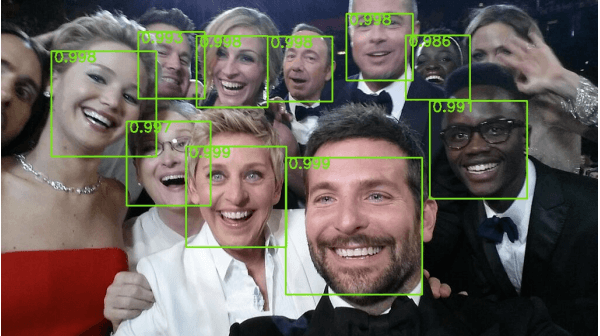
\includegraphics[scale=1]{img/figura-1.png}
 \textbf{Fonte:} Autor.
\label{fig:exemplo-vc}
\end{figure}



Os tópicos seguintes apresentam um panorama: da deficiência físico-motora, TA e o potencial da VC neste meio; a Metodologia utilizado neste trabalho, descrição e detalhamento do funcionamento do VisiUMouse até a fase de modelagem, Design entre outros.

%------------------------------------------------------------------

\chapter{PANORAMA DA DEFICIÊNCIA FISICO-MOTORA, TECNOLOGIA ASSISTIVA E POTENCIAL DA VISÃO COMPUTACIONAL}
\label{CAP2}

A evolução continua e exponencial das Tecnologias possibilitam cada vez mais a criação e melhorias de em vários âmbitos sociais, digitais, acadêmicos e profissionais. O qual cada indivíduo tem acesso a um arsenal de conhecimento imensurável, na \textit{internet}, como a grande quantidade de Artigos e pesquisas acadêmicas publicados diariamente e o desenvolvimento e distribuição continuo de \textit{softwares} de código aberto. É evidente o crescimento das possibilidades em todas as áreas de conhecimento com a revolução da informação, representado um novo modelo de mundial para todas as pessoas.


\section{A DEFICIÊNCIA NO BRASIL}\label{Sub:deficiencia-brasil}

Este arsenal possibilita que parte da população consiga atingir seus objetivos com maior facilidade e rapidez, apenas com um computador e acesso \textit{internet}, porém é diferente para um determinado tipo de público. Este público representa pessoas que manifestam algum tipo de deficiência, segundo (IBGE, 2010) cerca 23,9\% apresentam algum tipo de deficiência, este valor relata 45,6 milhões de Brasileiros em 2010, deste total 7\% apresentam deficiências motoras que englobam desde restrições suaves até outras severas, estas esferas de indivíduos com condições singulares equivalem a cerca de 3,192 milhões de pessoas só no Brasil. 
Pode definir deficiência como toda perda ou anomalia de uma estrutura ou função psicológica, fisiológica ou anatômica que gere incapacidade para o desempenho de atividade, dentro do padrão considerado normal para o ser humano \citeonline{brasil1999decreto}.

\section{TECNOLOGIA ASSISTIVA}\label{Sub:ta-brasil}
Os recursos e serviços que contribuem para proporcionar ou ampliar habilidades funcionais de pessoas com deficiência e consequentemente promover vida independente e inclusão é determinado de TA. A TA é uma expressão nova, que se refere a um conceito ainda em pleno processo de construção e sistematização. A utilização de recursos de TA, entretanto, remonta aos primórdios da história da humanidade ou até mesmo da pré-história. Qualquer pedaço de pau utilizado como uma bengala improvisada, por exemplo, caracteriza o uso de um recurso de TA \citeonline{galvao2009tecnologia}.

Este tipo de usuário encontra grande dificuldade em utilizar um computador pessoal, pelo fato de ser controlado basicamente apenas pelo movimento das mãos, membros estes dos quais podem ter sido atendidos pela deficiência, privando o usuário de mobilidade. Este motivo incapacita a utilização de dispositivos de entrada tradicionais, como o \textit{mouse} e teclado. Para este usuário uma tarefa simples de navegar na \textit{internet} para estudar se torna um desafio intangível, atenuado apenas pelas TAs disponíveis no mercado. São poucas as Tecnologias que dão suportem a casos onde o usuário tem apenas o controle do movimento da cabeça. Em muitos destes casos a pessoa deficiente possui as faculdades mentais intactas.

Para uma pessoa com deficiência, a simples tarefa de navegar na \textit{internet} torna-se um desafio quase intransponível, apenas amenizado pelas TA disponíveis no mercado. Poucas Tecnologias abrangem casos em que existe a perda completa do movimento dos membros. Nestes casos específicos de deficiência, normalmente, a única parte do corpo que o usuário consegue movimentar livremente são os olhos. Em muitos destes casos a pessoa deficiente possui as faculdades mentais intactas.

Estes fatos possibilitam que o usuário interaja com o seu ambiente apenas com a cabeça, como falar com pessoas. Essa condição determina que para ele utilizar um dispositivo eletrônico ele pode usar essencialmente a cabeça. Isto é o computador ou disposto precisa entender as expressões da cabeça e seus elementos, como boca, nariz e olhos, além da fala. Considerando estes fatos podemos citar três tipos de entrada de dados. A entrada de vídeo, onde o usuário vai estar disposto na frente de uma câmera como a \textit{webcam}. A entrada de áudio, onde o usuário vai precisar ter um microfone. E por fim a entrada de contato físico, onde o usuário vai precisar apertar botões, que estes casos devem ser grandes. 

\section{VISÃO COMPUTACIONAL}\label{Sub:vc}
Considerando estas entradas de dados é possível analisar que a entrada de vídeo possibilita uma interseção mais natural, considerando que o movimento da cabeça deve ser similar ao movimento da mão quando um usuário sem deficiência utiliza o \textit{mouse}.

Estas condições demostram que a interação com computador através do movimento da cabeça é justificável. Dentro da área da Computação dentro da IA existe uma subárea denominada VC, que tem como objetivo dar significado as imagens digitais com base em análise. Esta análise procura extrair algum conhecimento da representação matricial das imagens. Ou seja os estudos, \textit{softwares}, conceitos e aplicações podem dar significado a movimentação dos membros de qualquer pessoa. 

Estes desafios tornam-se complexos pelo fato das imagens digitais serem apenas visíveis para o computador, frequentemente são estrutura de dados no formato de matrizes de distribuição de pontos e também pelo fato de não armazenarem informações sobre a cena representada pela imagem, isto é meta dados. 

Um vídeo pode ser considerado um conjunto de imagens digitais, que é uma representação numérica de uma imagem bidimensional em forma binário, tornando possível o armazenamento, transferência, processamento ou reprodução por meios eletrônicos. Existe dois tipos de imagens, as imagens de rastreio (ou raster) e as imagens do tipo vetorial.

As imagens de rastreio são representadas de forma matricial pelo computador, onde há uma correspondência bit-a-bit da matriz que representa a imagem como o que está sendo reproduzido de fato tela. A resolução de uma imagem defini a sua matriz, então uma imagem de 1024x720 tem 737280 posições em uma matriz. As matrizes deste tipo não possuem nem um tipo de dados adicionais como o que existem na imagem ou que tipo de objetos ele representa. A representação e extração destes dados é tarefa da área de VC, que tem como objeto dar significado semântico para imagens digitais através do processamento delas, de acordo com \citeonline{prince2012computer}. Uma das técnicas para detectar objetos em uma imagem digital é o algoritmo de Viola-Jones, que foi utilizado no VisiUMouse.

\subsection{Conceito de Viola-Jones}
O algoritmo de Viola-Jones para a identificação de objeto é um algoritmo proposto para o reconhecimento de objetos em imagens digitais, e tem como característica o alto desempenho de processamento e o alto indicie de assertividade, podendo chegar até a 99,7\% dependendo do número de etapas treinadas, acurácia do classificado e objeto para qual foi treinado \citeonline{viola2001rapid}. O qual trabalha com algoritmo em cascata que se utiliza de arquivos de padrões e características chamados de haar fea-tures. Estas características são organizadas em uma estrutura de árvore em XML.

\subsection{OpenCV}
O OpenCV (\textit{Open Source Computer Vision Library}) é uma biblioteca multiplataforma desenvolvida pela Intel Corporation, que implementa diversos módulos para VC, este os quais são utilizados para o Processamento de Imagens e Vídeo, Estruturas de dados, álgebra linear e mais de 350 algoritmos de VC. OpenCV possui, em seu módulo central uma implementação do algoritmo de Viola-Jones para detecção de objetos. 

\chapter{METODOLOGIA}\label{CAP3}
O projeto desenvolvido propõe o uso de VC para a criação de um sistema capaz de identificar e rastrear os olhos do usuário e a partir disto dar controle sobre o seu computador através da simulação de um \textit{mouse} comum.
	O desenvolvimento deste projeto tem como objetivo permitir que usuários com algum tipo de deficiência físico-motora consiga operar seu computador doméstico de forma simples e fácil apenas com a cabeça. Para isto foi necessário fazer uma pesquisa de possíveis Tecnologias, estudos relacionados e teste para   determinar a viabilidade do desenvolvimento do projeto proposto.
    
\section{TRABALHOS RELACIONADOS}\label{Sub:trabalhos-relacionados}
Existem vários tipos de  \textit{software} de TA, e a seguir são apresentados um resumo de alguns dos \textit{softwares} difundidos no meio. Parte dos \textit{softwares} de TA são utilizados para a comunicação com outras pessoas, geralmente o seu responsável, porém existe outros \textit{softwares} que tem como objetivo a independência que permite que seus usuários exerçam atividades sozinhos ou com pouca ajuda. 

Existem diversos projetos, produtos e estudos em TA, baseados na VC, que utilizam-se de \textit{softwares} para detecção de objetos através de uma \textit{webcam} \cite{ramos2016letras,gips2000camera,bian2016facial,marnik2014blinkmouse}. A detecção dos movimentos nesses projetos é feita através de uma entrada de vídeo que rastreia várias partes do corpo humano, sendo que a mais comum é o rastreamento de movimentos da cabeça (\textit{video-based}) \cite{al2013eye}. 

%O objetivo dos trabalhos relacionados 
Um dos objetivos de análise desses trabalhos é não depender de dispositivos de alto poder computacional, utilizando Tecnologias disponíveis no próprio computador. Das soluções \textit{video-based} a mais adotada é o \textit{software} CameraMouse \cite{gips2000camera} que frequentemente é usado como base de pesquisas e de comparações, como em Kurauchi \cite{kurauchi2015hmagic}. A seguir são apresentados um resumo de alguns dos \textit{softwares} difundidos no meio.

\subsection{CameraMouse}
O \textit{software} CameraMouse é capaz de capturar o movimento dos olhos ou qualquer outra parte do corpo com que se queira manipular o \textit{mouse} do computador. O sistema foi desenvolvido para trabalhar com a plataforma Windows e seu funcionamento se dá através dos recursos do \textit{webcam}. O programa foi desenvolvido para ajudar as pessoas com deficiência e o principal público-alvo deste \textit{software} são as pessoas que não têm controle confiável das mãos, mas que podem executar movimentos com a cabeça \citeonline{gips2000camera}.

Dentre os softwares similares este é o mais semelhante a Tecnologia VisiUMouse, usando dos mesmo conceitos e princípios da VC. A Figura \ref{fig:camera-mouse} apresenta a tela inicial do CameraMouse, o quadrado pequeno na cor verde posicionado no nariz da pessoa representa a área que o usuário selecionou para o \textit{software} rastrear, forçando o usuário estar sempre na mesma posição, podendo apenas mover sua cabeça em inclinar para os lados, forçando o usuário a fazer movimento espelhados  e assim causando um maior esforço do usuário. O CameraMouse não possibilita usar a inclinação da cabeça para controlar o \textit{mouse}, isto é, para o usuário mover o ponteiro ele preciso imaginar que na tela do computar existe um espelho e que ele deve posicionar o quadrado verde na área que deseja.

\begin{figure}[htbp]
\caption{Tela inicial do Software CameraMouse.} 
\centering 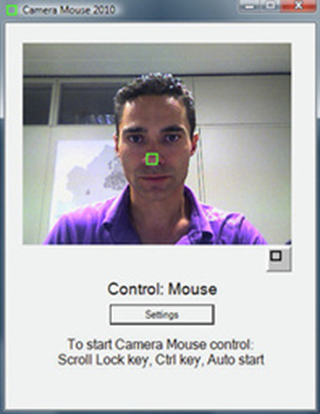
\includegraphics[scale=1]{img/camera-mouse.png}

\textbf{Fonte:} Autor.
\label{fig:camera-mouse}
\end{figure}

\subsection{HeadDev}
O projeto HeadDev \citeonline{alvesferramentas} é semelhante ao CameraMouse, porém faz o rastreamento apenas dos movimentos da cabeça, não permitindo configurar o objeto que o \textit{software} deve rastrear. Seu funcionamento também utiliza a técnica de espelhamento.

\subsection{Facial Mouse}

Facial Mouse é uma interface de IHC para as pessoas com tetraplegia baseada em uma câmera de profundidade de infravermelho monocular. A posição do nariz junto com a boca é detectado para o controle e navegação do cursor do \textit{mouse}. O algoritmo utilizado para rastrear é baseado em uma árvore melhorada de decisão aleatória que é capaz de detectar a informação facial de forma eficiente e com precisão. Com isso é possível uma experiência melhor para o usuário, tornando mais confortável o alcance do movimento do nariz para o movimento do cursor através de uma função não-linear. A câmera de profundidade infravermelha permite o sistema ser independente de iluminação e mudanças de cor tanto o fundo e no rosto humano, o que é uma vantagem crítica
So  bre as opções baseadas em câmera RGB \citeonline{bian2016facial}.

\subsection{Facial Human-Computer Interface e BlinkMouse}
Já os \textit{softwares} Facial Human-Computer Interface \citeonline{antunes2016intelligent} e BlinkMouse \citeonline{marnik2014blinkmouse} tem como objetivo aplicar o modo de interação feita pelo CameraMouse, refinando a funcionalidade do clique, principalmente nos requisitos de precisão e configuração.

%@IMPORTANTE
Baseado nos trabalhos relacionados percebe-se a utilização dos conceitos de VC e o uso da OpenCV, com a técnica de espelhamento do movimento e rastreamento da face principalmente. Nesse contexto o VisiUMouse tem como um dos objetivos implementar uma técnica de movimento alternativa, batizada de Técnica de Zona Neutra e de Movimento (TZNM) \citeonline{xavier2017visiumouse}, com o rastreamento dos olhos para o controle do ponteiro, facilitando  um implementação futura de clique pelo piscar dos olhos e \textit{Eye Tracking}.

\section{VIABILIDADE}\label{Sub:viabilidade}
Com a crescente evolução das áreas de IA é evidente o aumento de ferramentas e estudos que colaboram para a criação e implementação de novas aplicações. Uma subárea da IA que vem ganhando destaque é a VC que tem como foco extrair significado as imagens virtuais com base em análise e estudo de padrões.

Com a evolução da VC possibilitou a criação de novas aplicações, toda atividade humana que tinha como base a visão pode ser transformada em uma aplicação de VC. Grandes inovações nas áreas de saúde e Astronomia com a ajuda desta área agora são possíveis, por exemplo. Atualmente é possível utilizar esta área para a busca de estruturas estranhas em imagens de exames de tomografia. 
    
O potencial e a evolução da VC perpetuam o aumento de novos estudo e ferramentas. OpenCV é uma biblioteca grátis e multiplataforma, isto é compatível com múltiplos Sistemas Operacionais e Linguagens de Programação, como Java e C\#, ele foi desenvolvido pela Intel Corporation, que implementa diversos módulos e cerca de 350 algoritmos de VC, e atualmente está presente em diversos \textit{software} e estudos, tornando as aplicações de VC mais acessíveis.  

Os fatores apresentados manifestam as possibilidades de criação de aplicações com base em VC, grande parte deste cenário é possível graças a biblioteca OpenCV que é uma biblioteca de código aberto e compatível com os principais Sistemas Operacionais e Linguagens de Programação do mercado. Estes fatores determinam a escolha dela e da Linguagem de Programação Java para o desenvolvimento trabalho proposto. Assim como a maioria das Linguagens de Programação a Java não gera custos.

O trabalho proposto tem como público-alvo pessoas com algum tipo de deficiência motora ou física, que possuem o movimento da cabeça e com a capacidade cerebral preservada. O  censo do IBGE de 2010 no Brasil indica que existem cerca de 45,6 milhões de pessoas com deficiência \citeonline{IBGE:2010}, representando 23,9\% da população brasileira; deste total 7\% apresentam deficiências motoras que englobam desde restrições suaves até outras severas, estas esferas de indivíduos com condições singulares equivalem a cerca de 3,192 milhões de pessoas no Brasil em 2010.

Os fatores apresentados e a experiencia adquirida em outros projetos relacionados com acessibilidade e TA evidenciam aspectos para a viabilidade do trabalho apresentado. Entre as experiencias podemos citar a quantidade de usuários com deficiência físico-motora no Brasil e na região de Pelotas; de instituições que amparam esses usuários as quais podem ser abordadas diretamente para apresentar O VisiUMouse; que boa parte desses usuários não estão presentes diretamente na sociedade, tendo em vista que eles representam cerca de 7\% da população.

\chapter{VISIUMOUSE}\label{CAP4}
VisiUMouse é um projeto de VC com o objetivo de ajudar pessoas com algum tipo de deficiência físico-motora a utilizar o computador de maneira simples e fácil apenas com do movimento da cabeça, usando os olhos como referencia. Permitindo a substituição do \textit{mouse} comum por um nova interface homem-computador adequada e configuráveis. O rastreamento dos olhos do usuário é sutil e não causa nem um desconforto, e apresenta vantagens óbvias para usuários humanos que não podem usar dispositivos tradicionais de entrada de computador, como teclado, \textit{mouse} e teclado. Este tipo de Tecnologia tem outro diferencial que é desnecessário um \textit{hardware}, sensor, sinal conectado no usuário.

\section{Funcionamento}\label{Sub:funcionamento-visiumouse}
VisiUMouse é um projeto que tem como objetivo principal a utilização de Computadores Pessoais (PC) exclusivamente com o movimento da cabeça, isto é possível com base na captura de vídeo feita pelo \textit{webcam} do usuário e o processamento dos dados do vídeo recebidos, e com o uso de algoritmos de rastreamento de objetos e \textit{Machine Learning} é possível reconhecer a posição atual dos olhos do usuário. 

O processo de \textit{machine learning} é utilizado para reconhecer padrões de formas de objetos, neste caso foi para reconhecer olhos humanos, para isso foi necessário utilizar um banco de dados com grande volume de imagens de olhos que gerou um arquivo XML com estes padrões. Com o arquivo XML com os padrões foi utilizado os conceitos do algoritmo de Viola-Jones para fazer o processo de rastreamento \citeonline{viola2001rapid}. Este arquivo XML contém os padrões e características são chamados de \textit{haar fea-tures}, que são uma lista de características invariantes de um objeto.

Os objetos procurados pela estrutura de detecção universalmente envolvem as somas de pixels de imagem dentro de áreas retangulares, estes valores são comparados com os valores dos estágios do arquivo \textit{haar fea-tures}, e assim determinar se a área examinada da imagem possui ou não o objeto que pretende detectar.  A Figura \ref{fig:viola-jones-ret} apresenta o processo de somas de pixels da imagem que está sendo trabalhada, as somas são feitas dentro dos retângulos. 

\begin{figure}[htbp]
\caption{Algoritmo de Viola Jones.} 
\centering 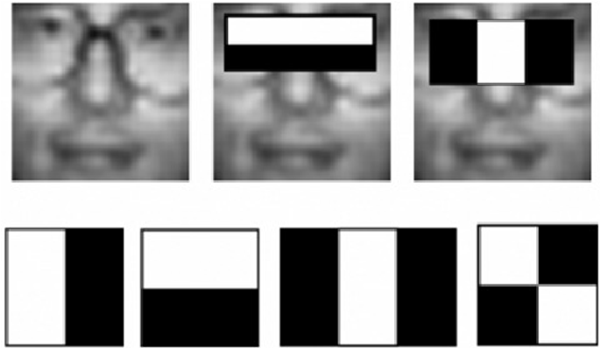
\includegraphics[scale=1]{img/viola-jones-ret.png}
\textbf{Fonte:} Autor.
\label{fig:viola-jones-ret}
\end{figure}

Aplicação de rastreamento dos olhos foi desenvolvida usando a linguagem de programação Java, esta linguagem oferece um arsenal de bibliotecas para PDI e o suporte a desenvolvimento de sistemas multiplataforma, isto é, funciona em diferentes Sistemas Operacionais. 

Normalmente os processos de rastreamento são feitos em um processador responsável pela renderização de gráficos em tempo real. Este tipo de processador é chamado de \textit{Graphics Processing Unit}, também conhecido como GPU.

Genericamente o processamento da imagem contém 3 estágios: Captura, Análise e Compressão da Imagem. A \textbf{Captura} trata da aquisição dos dados de entrada de vídeo; a \textbf{Análise} trata do reconhecimento do objeto alvo. Para o reconhecimento é necessário um conjunto de padrões do alvo, esse processo é nomeado de Treinamento e é responsável por gerar um arquivo XML que contém características e padrões dos objetos alvos. A Classificação é o processo final que define se um determinado pedaço da imagem contém o objeto que pretende detectar. A \textbf{Compressão da Imagem} é o processo feito para reduzir a redundância dos dados, de forma a armazenar ou transmitir esses mesmos dados de forma eficiente. \citeonline{rolim2008sistema}.

Com os conceitos do algoritmo de Viola-Jones e as bibliotecas de suporte a PDI foi possível desenvolver o VisiUMouse, o qual tem como característica principal o reconhecimento e rastreio dos olhos de qualquer pessoa para dar-lhe o controle do \textit{mouse}, o processo de movimento dos olhos e o movimento do ponteiro do \textit{mouse} é dado em dezenas de milissegundo, este valor do tempo depende da GPU do computador do usuário, com o sistema também desenvolvido o simulador de \textit{mouse}. A Figura \ref{fig:visiumouse-1} mostra o funcionamento do rastreando dos olhos do usuário.

\begin{figure}[htbp]
\centering
\caption{MVP do VisiUMouse.}
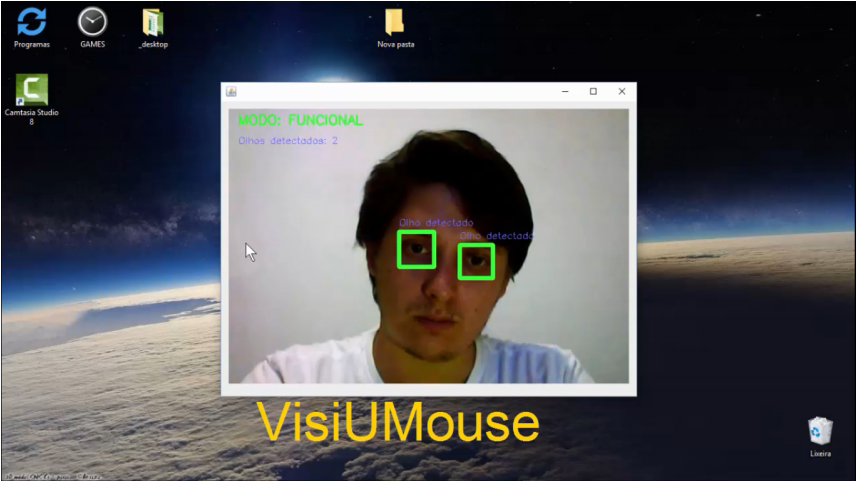
\includegraphics[scale=.6]{img/visiumouse-1.png}

  \textbf{Fonte:} Autor.
\label{fig:visiumouse-1}
\end{figure}

O VisiUMouse tem seu funcionamento baseado no movimento da cabeça/face, usando os olhos como ponto de referencia e a Técnica de Zona Neutra e de Movimento (TZNM). A medida do deslocamento dos olhos é feita através do processamento da posições anteriores, ou seja, se a medida for superior a configurada é feita a movimentação do ponteiro (zona de movimento da TZNM), se for menor o ponteiro permanece parado (zona neutra da TZNM). Para processar para qual lado o cursor deve ir é verificada a posição dos olhos em relação às linhas (ilusórias) vermelha e verde, como pode ser visto na Figura \ref{fig:funcionamento}.

\begin{figure}[htbp]
\caption{Layout do VisiUMouse: telas de rastreamento e processamento do deslocamento dos olhos.}
\centering 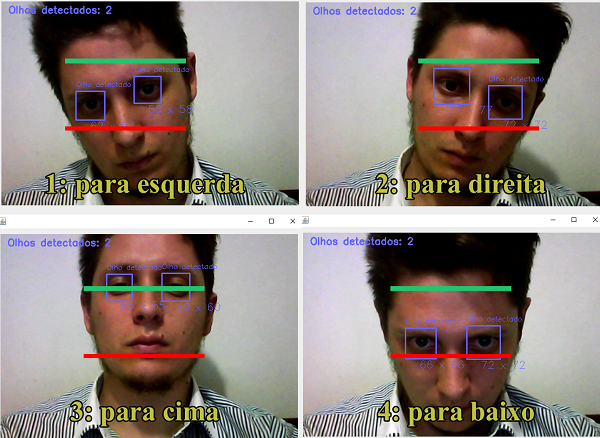
\includegraphics[scale=1]{img/funcionamento2.png}
\textbf{Fonte:} Autor.
\label{fig:funcionamento}
\end{figure}

Para determinar a direção do movimento do ponteiro é feita uma comparação com a posição dos olhos em relação às linhas verde e vermelha. Por exemplo, se o olho direito estiver próximo da linha verde e o olho esquerdo próximo da linha vermelha, indica que o usuário está com a cabeça inclinada para esquerda e que o cursor do \textit{mouse} deve ir para o mesmo lado, como mostrado na Figura \ref{fig:funcionamento} (1: para esquerda). Também é possível fazer movimentos para direita, para cima e para baixo (vide Figura \ref{fig:funcionamento}), além da combinação desses movimentos, tornando possível realizar movimentações em diagonal. No momento em que o movimento do cursor do \textit{mouse} se inicia, o usuário não precisa mais deslocar os olhos para manter o movimento, ele apenas precisa permanecer na mesma posição, podendo tornar o controle do \textit{mouse} menos cansativo, e assim evitando o desgaste físico do usuário \footnote{Foi disponibilizado um vídeo com o funcionamento básico do VisiUMouse, em: http://visiumouse.com/\#funcionamento}. 

\subsection{Tabela Comparativa}\label{Sub:tabela-comparativa}
A área de TA apresenta um número significativo de Tecnologia que permitem o melhor uso de um Computador e comunicação, algum desses tem como objetivo ajudar na formulação de frases através de um teclado com imagens que representam palavras comuns, como: comer, água, banheiro, música etc. Outra parte dessas Tecnologias tem como objetivo viabilizar o uso do Computador sem ajuda de outras pessoas, geralmente essas Tecnologias apresentam controles de acionamento mecânico como grandes pedais ou palancas, entra elas ainda existe  um tipo de Tecnologia que permite o uso do Computador apenas com o movimento da cabeça, geralmente a leitura do movimento é feito por um  entrada de vídeo que filma e interpreta seus movimentos.

A Tabela \ref{tabela-comparativa} apresenta uma comparação entre os \textit{softwares}: VisiUMouse, CameraMouse e FacialMouse; os quais apresentam algumas semelhanças como: \textit{webcam} como entrada de vídeo, uso da biblioteca OpenCV e do algoritmo de Viola-Jones. O CameraMouse é usado em diversas pesquisas, tendo mais de mil resultados no Google Acadêmico. O FacialMouse apresenta um refinamento em suas funcionalidades comparado ao CameraMouse. O CameraMouse e FacialMouse são um dos poucos que estão disponível para download, é difícil o acesso as TA, grande parte são presente apenas em artigos acadêmico, são poucas as que estão disponíveis para o publico, além disso elas ainda não difícil de encontrar, algumas por terem nomes genéricos outras por terem sites não ranqueado em motores de  busca como Google.

A Tabela \ref{tabela-comparativa} apresenta 6 atributos de comparação:
\begin{enumerate}
\item \textbf{Click por Tempo}: as Ta com base em vídeo geralmente utilizam a técnica do click do \textit{mouse} para simplificar o uso, esta técnica consiste em deixar o cursor do \textit{mouse} parado por um determinado tempo para gerar o click na mesma posição que o curso esta. Apesar do Click por Tempo ser comumente utilizado pode influenciar no desempenho do usuário em executar tarefas no computador que necessitam ser rápidas, como jogos. O VisiUMouse faz o rastreamento dos olhos permitindo implementar uma funcionalidade de click pelo piscar dos olhos. 
\item \textbf{Tipos de Clicks}: este atributo representa a variedade de tipos de clicks e funcionalidade do \textit{mouse} que a Tecnologia apresenta, entre eles estão o Click Primário (comumente o botão esquerdo do \textit{mouse}), click secundário (comumente o botão direito do \textit{mouse}), a funcionalidade de arrastar etc.
\item \textbf{Multiplataforma}: característica de um sistema funcionar igualmente em diferentes plataformas (Sistemas Operacionais).
\item \textbf{Tipo de Movimento}: atributo que define como o movimento do cursor é feito em ralação ao objeto rastreado. As TA apresentadas utilizam o movimento espelhado que pode ser determinado por um reflexo do movimento do objeto rastreado no moimento do cursor do \textit{mouse}, apesar de ser intuitivo pode causar um desgaste físico extra na região do pesco e tornar inviável para pessoas que tenham menos mobilidade com a cabeça. A TZNM apresenta uma solução alternativa para o movimento do cursor do \textit{mouse} possibilitando um desgaste físico menor e o movimento por toda a tela do computador com uma menor mobilidade da parte do usuário.
\item \textbf{Objeto Rastreado(s)}: atributo que define qual objeto da cabeça do usuário é rastreado, ou seja o objeto que o \textit{software} vai identificar a cada \textit{frame} da entrada de vídeo para definir o deslocamento desse objeto. O CameraMouse permite um configuração de qual objeto vai ser rastreado, porém perde a referencia com algum tempo de uso fazendo com que o usuário precise configurar de novo o objeto. Já o FacialMouse rastreia o rosto do usuário permitindo que o usuário não precise fazer um configuração antes de usar. O VisiUMouse rastreia os 2 olhos do usuário possibilitando 2 pontos de referencia que podem aumentar a precisão da leitura dos movimentos do usuário.
\item \textbf{Quantidade Objeto Rastreado(s)}: define a quantidade de objetos que sera rastreado, quanto maior a quantidade mais pontos de referencia o sistema vai ter para entender o movimento do usuário.
\end{enumerate}







%https://www.tablesgenerator.com/
% Please add the following required packages to your document preamble:
% \usepackage[table,xcdraw]{xcolor}
% If you use beamer only pass "xcolor=table" option, i.e. \documentclass[xcolor=table]{beamer}
\begin{table}[tbp]
\centering
\caption{Tabela Comparativa}
\label{tabela-comparativa}
\begin{tabular}{|l|l|l|l|}
\hline
\multicolumn{1}{|c|}{\textbf{Tecnologia,Assistiva}} & \multicolumn{1}{c|}{\textbf{VisiUMouse}} & \multicolumn{1}{c|}{\textbf{CameraMouse}} & \multicolumn{1}{c|}{\textbf{Facial Mouse}} \\ \hline
Click por Tempo                                     & \cellcolor[HTML]{67FD9A}Sim              & \cellcolor[HTML]{67FD9A}Sim                & \cellcolor[HTML]{67FD9A}Sim                \\ \hline
Tipos  de Clicks                                    & Principais                               & Principais                                 & Esquerdo                                   \\ \hline
Multiplataforma                                     & \cellcolor[HTML]{67FD9A}Sim              & \cellcolor[HTML]{67FD9A}Sim                & \cellcolor[HTML]{67FD9A}Sim                \\ \hline
Tipo de Movimento                                   & TZNM                                     & Espelhado                                  & Espelhado                                  \\ \hline
Objeto Rastreado(s):                                & Olhos                                    & Selecionavel                               & Rosto                                      \\ \hline
Quantidade de Objetos Rastreados:                   & 2                                        & 1                                          & 1                                          \\ \hline
\end{tabular}
\end{table}

\chapter{MODELAGEM}\label{CAP5}
A modelagem de \textit{software} é de extrema importância por que determina as necessidades de um sistema de informação. E determina os questionamentos que vão mapear a estrutura do sistema, como “Qual a real necessidade de se projetar este sistema? ”, existe uma diferença importante entre a modelagem e a prática da construção do sistema, isto é o desenvolvimento. Os 2 devem trabalhar juntos para o bem te todas as partes de um \textit{software}, tanto cliente quanto empresa ou desenvolvedor. E para fazer a modelagem se utiliza de diagramas que é o próximo tópico deste documento.

\section{DIAGRAMAS}\label{Sub:diagramas}
Foram utilizados os conceitos de Linguagem de Modelagem Unificada (UML) apresentados em aula na disciplina de Análise e Projeto Orientados a Objetos para a modelagem dos diagramas. Através deles foi possível ter uma visão mais refinada do funcionamento do sistema e possível pontos instáveis do projeto, influenciando positivamente no desenvolvimento. A seguir serão apresentados os conceitos dos diagramas utilizados como Diagrama de Caso de Uso e Diagrama de Sequência, e após serão mostrados os diagramas e a estrutura conceitual básica de funcionamento do sistema. 

\subsection{Diagrama de Caso de Uso}
O Diagrama de Caso de Uso utiliza a linguagem simples, descrevendo o comportamento externo do sistema, apresentando o sistema através de uma perspectiva do usuário, demonstrando as funções e funcionalidades disponíveis para o usuário. Este diagrama é o mais abstrato, flexível e informal, sendo o utilizado com mais frequência na modelagem de sistemas, sendo uma base confiável para a modelagem, segundo \citeonline{guedes2011uml}. 

A Figura \ref{fig:use-case-diagram} mostra o Caso de Uso do sistema desenvolvido, a funcionalidade dele é relativamente simples, no diagrama temos dois Atores. O Ator “usuário” é o usuário que vai utilizar o computador apenas com o movimento dos olhos, ele é o foco deste projeto. O Ator “responsável” que pode ser definido como a pessoa responsável por cuidar do usuário, podendo ser algum familiar ou profissional da área da saúde como enfermeiro(a) ou médico(a), ele vai ser responsável por apenas executar a aplicação, isto é, ele só é necessário no primeiro momento. 

O início do funcionamento é marcado pela a inicialização da aplicação, representado como a elipse “iniciar aplicação” no diagrama. Em seguida o sistema se encarrega de fazer o reconhecimento dos olhos, representado pela elipse “reconhecimento olhos” no diagrama, o sistema ainda define qual das duplas de olhos ele deve rastrear, esta funcionalidade é representada pela elipse “definir olhos principais” no diagrama.  Após isto é dado o controle do \textit{mouse} para o usuário, é feita uma simulação do \textit{mouse}, representado pela elipse “controlar mouse”, além disto é possível entrar na área de configuração a qualquer momento, representado pela elipse “configurar”.

\begin{figure}[htbp]
\caption{Diagrama de Caso de Uso.}
\centering 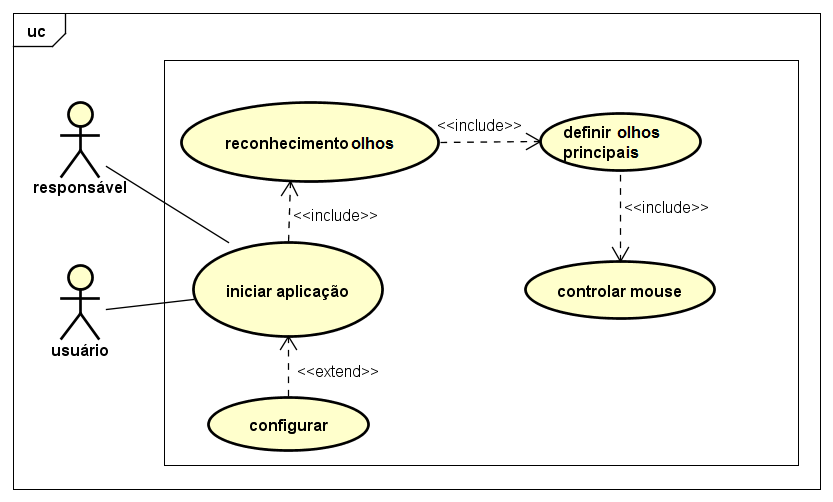
\includegraphics[scale=.6]{img/UseCase_Diagram_2.png}

\textbf{Fonte:} Autor.
\label{fig:use-case-diagram}
\end{figure}

\subsection{Diagrama de Classes}
O Diagrama de Classes é o mais utilizado e o mais importante da UML. É extremamente relevante junto com o paradigma de Orientação a Objetos. E serve de apoio para a maioria dos demais diagramas. Como o próprio nome diz, define a estrutura das classes utilizadas pelo sistema, determinando os atributos e métodos que cada classe possui, segundo \citeonline{guedes2011uml}. O Diagrama da Figura \ref{fig:diagrama-classes} apresenta o diagrama utilizado para modelagem do sistema, a classe “Detector” tem grande destaque na funcionalidade do sistema, é ela que detecta e rastreia os olhos do usuário, ela está representada no diagrama como “Detector”. Outra classe importante é a responsável por simular o \textit{mouse}, dando o controle do computador para o usuário, está representado como “Mouse” no diagrama. E por fim a classe “Main” que é a responsável por controlar as outras classes. 

\begin{figure}[htbp]
\caption{Diagrama de Classes.} 
\centering 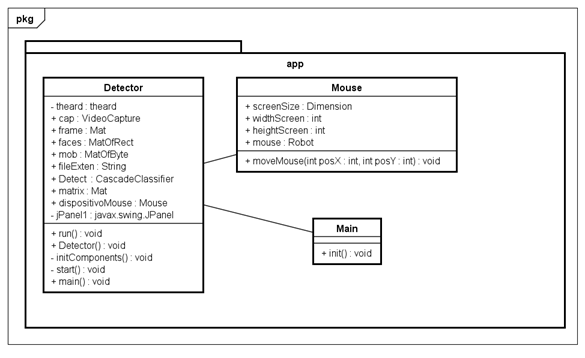
\includegraphics[scale=1]{img/diagrama-classes.png}
\textbf{Fonte:} Autor.
\label{fig:diagrama-classes}
\end{figure}


\subsection{Diagrama de Sequência}
O Diagrama de Sequência apresenta a ordem temporal em que as mensagens são trocadas entre os objetos envolvidos em uma determinada função. Em geral, baseia-se em um Caso de Uso definido pelo diagrama de mesmo nome e tem como base o Diagrama de Classes para determinar os objetos das classes envolvidas em um processo, segundo \citeonline{guedes2011uml}. A Figura \ref{fig:diagrama-sequencia} apresenta o Diagrama de Sequência do sistema.

O início da representação temporal do diagrama é dada pela ação do Ator “Usuário”, no momento que ele iniciar a aplicação “1.1 init app()” o sistema já vai começar a detectar os olhos na entrada de vídeo, ou seja no momento que o programa foi executado a entrada de vídeo (\textit{webcam}) estiver fornecendo dados o sistema vai detectar todos os olhos presentes no vídeo. Quando o sistema identifica mais de uma dupla de olhos ele determina qual delas deve rastrear e usar para controlar o Computador, esta funcionalidade está representada no diagrama como “3.1 Detectar Olhos”. E na etapa final é dado o controle do computador para o usuário através da simulação das funcionalidades do \textit{mouse}, no diagrama está representado como “”3.2 Controlar mouse()”. 

\begin{figure}[htbp]
\caption{Diagrama de Sequencia.}
\centering 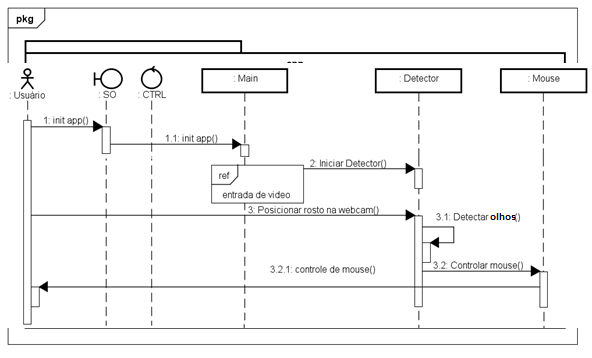
\includegraphics[scale=1]{img/diagrama-sequencia.png}
\textbf{Fonte:} Autor.
\label{fig:diagrama-sequencia}
\end{figure}

\chapter{DESIGN}\label{CAP6}
A importância do Design esta no desenvolvimento de produtos (digitais ou físicos) que facilitem a vida das pessoas ele possibilita criar coisas funcionais e bonitas. O Design pode dar destaque a um produto com as mesmas funcionalidade e preço de outros. Por isso o Design é o fator decisivo no sucesso ou fracasso de um produto. Assim como um Design bem pensado desperta o desejo dos consumidores, um Design pobre e mal feito gera uma repulsa enorme, segundo \citeonline{patterson2017computer}.

Este trabalho apresenta o Design do \textit{software} e site do VisiUMouse, o \textit{software} é um sistema \textit{desktop} que é executado pelo usuário na área de trabalho do Computador, permitindo que ele controle o Computador; o site é o responsável por apresentar e disponibilizar esse sistema na \textit{Web} para os usuários, entre outras funcionalidades.

\section{DESIGN DO SOFTWARE DESKTOP}\label{Sub:software}
Para a criação da interface foi utilizado os conceitos de CRAP (Contraste, Repetição, Alinhamento e Proximidade) apresentados na disciplina de Design de Interface, a escolha da paleta de cores foram definidas através de um levantamento das principais cores das Tecnologias Digitais atuais, foi feito uma pequena alteração nesta paleta para torná-la única e por consequência uma característica da própria Tecnologia, as outras estilizações como sombra e tipografia foram definidas através das tendências atuais. Além de seguir boa práticas de \textit{Graphical User Interface} (GUI) para pessoas com pouca mobilidade, por exemplo botões grandes e mais afastados. A Figura \ref{fig:interface-tecnologia} mostra a tela principal do \textit{software} VisiUMouse.

\begin{figure}[htbp]
\caption{Interface principal do VisiUMouse.} 
\centering 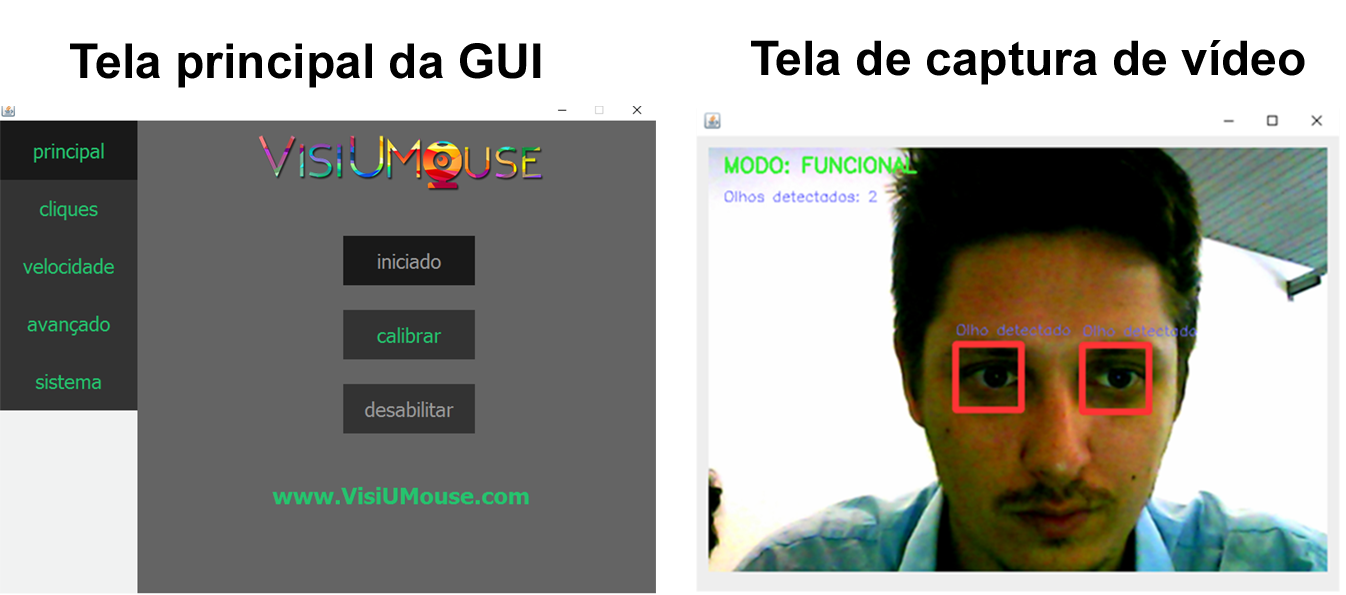
\includegraphics[scale=.3]{img/interface-tecnologia.png}

\textbf{Fonte:} Autor.
\label{fig:interface-tecnologia}
\end{figure}

\section{DESIGN DO SITE}\label{Sub:site}

O desenvolvimento do site tem como objetivo disponibilizar todo o conteúdo referente ao VisiUMouse, como o próprio \textit{software}, informações, módulos que foram criados juntamento com o VisiUMouse, uma página de contato entre outros. A Figura \ref{fig:site} apresenta a página inicial do site, no topo esta presente o menu de navegação que é fixo que permite que o usuário navegue entre todo o site de forma simples.

\begin{enumerate}
\item \textbf{inicial}: esta representado como a logo do site, do lado extremo esquerdo, ao clicar nessa imagem o usuário volta para o inicio da página.
\item \textbf{videos}: essa seção mostra um conjunto de vídeos que tem como objetivo dar uma visão geral do VisiUMouse
\item \textbf{funcionamento}: apresenta uma explicação resumida de como utilizar o VisiUMouse.
\item \textbf{contato}: nessa seção é possível enviar uma mensagem para o sistema.
\end{enumerate}


\begin{figure}[htbp]
\caption{Interface da página inicial do Site.} 
\centering 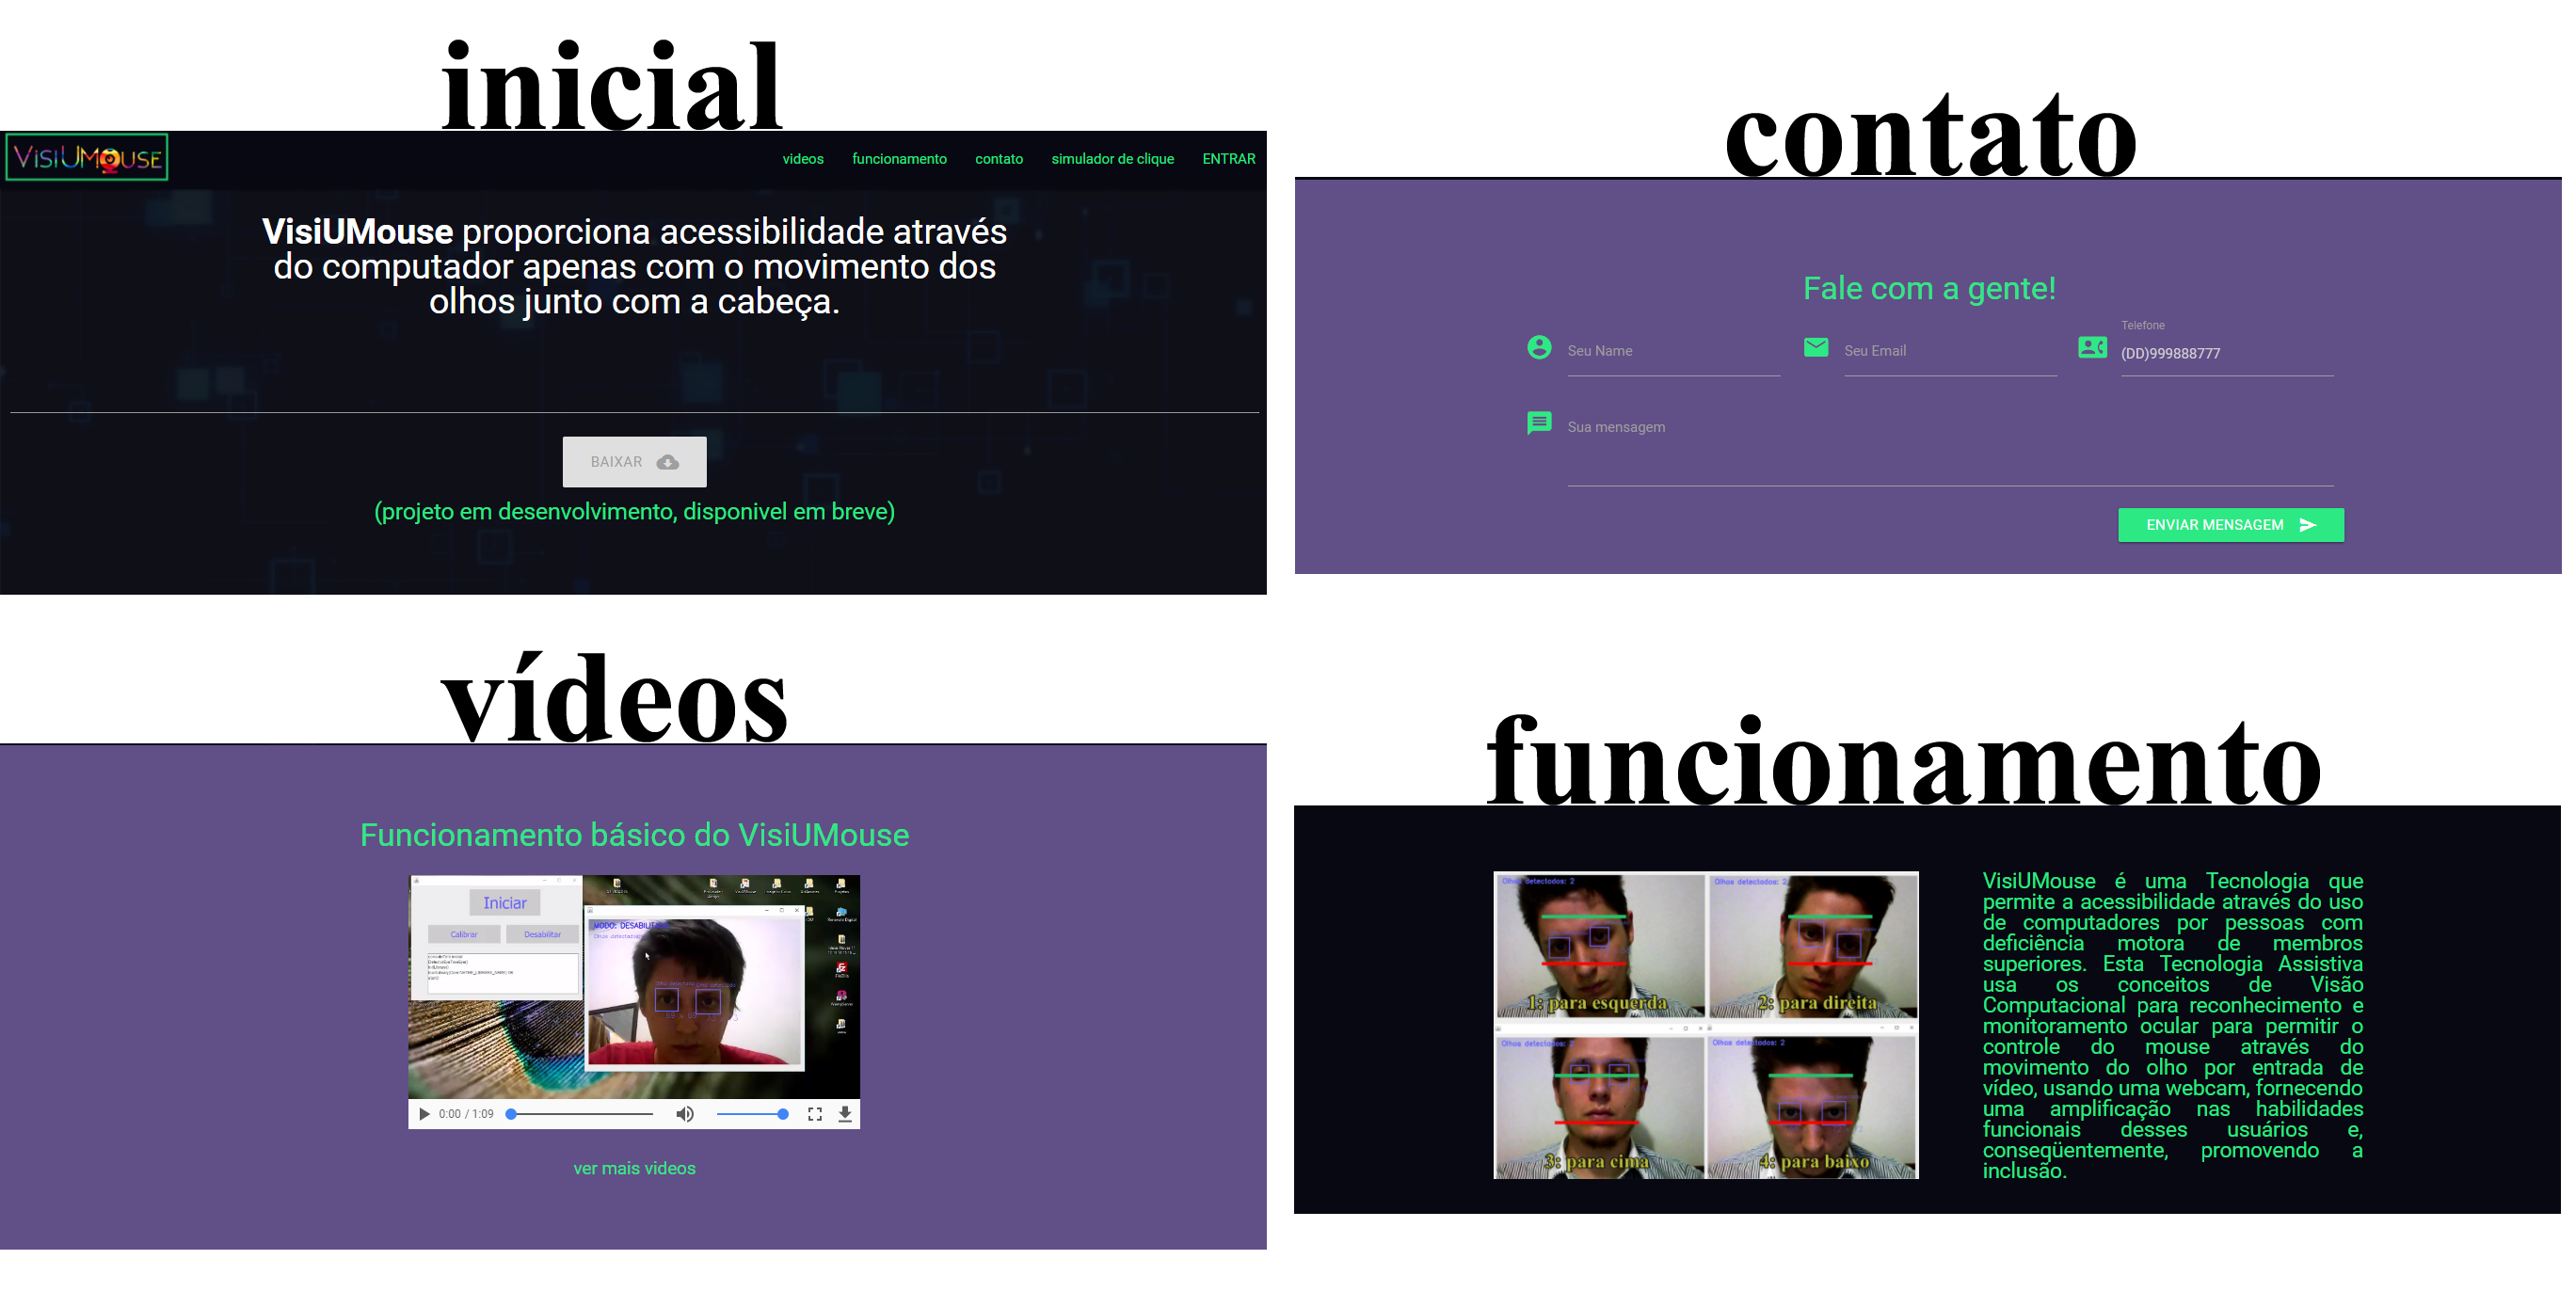
\includegraphics[scale=.165]{img/site.png}
\textbf{Fonte:} Autor.
\label{fig:site}
\end{figure}

\chapter{EXPERIMENTO 1}\label{CAP7}
O experimento foi executado por 9 participantes voluntários e teve como objetivo fazer uma avaliação comparativa do \textit{software} VisiUMouse com o \textit{mouse} convencional para avaliar o seu funcionamento e objetivo. Para tanto foi utilizado um protocolo baseado na lei de Fitts, proposto por \citeonline{soukoreff2004towards}, envolvendo tarefas comuns como apontar, selecionar e clicar, que são usadas como métricas para verificar a interação com o Computador. O protocolo foi configurado para 6 etapas, com 5 alvos cada, podendo ter o tamanho de 120, 150 ou 180 \textit{pixels}. O tamanho (gerados aleatoriamente) de cada um dos 5 alvos são iguais para cada fase \footnote{Foi disponibilizado gravações dos testes em: http://visiumouse.com}.

O teste foi dividido em 3 etapas: a primeira consistiu na aprendizagem de uso da aplicação, onde o participante era familiarizado com o funcionamento do VisiUMouse durante 5 minutos; a segunda etapa consistiu no experimento em si com o VisiUMouse; na última etapa, o participante utilizou o \textit{mouse} convencional para a execução das mesmas tarefas da etapa anterior. Os resultados são computados pelo \textit{software} do protocolo.

Para as três etapas foi utilizado o clique por tempo, denominado \textit{dwell time}, segundo \citeonline{gips2000camera}, configurado para o tempo 5 segundos para efetuar o clique. Cabe ressaltar que em paralelo ao desenvolvimento do VisiUMouse foi criado um sistema de clique por tempo para ser usado nos testes \footnote{Sistema de clique por tempo. Disponível em: http://visiumouse.com}. As demais configurações do VisiUMouse como velocidade foram mantidas iguais em todos os testes.  

O experimento foi conduzido com um notebook (LG S460) equipado com Windows 10, processador 2,4GHz (i3), 4 GB RAM, monitor de 14 polegadas, resolução de 1366 x 768 \textit{pixels} e utilizou-se a \textit{webcam} do próprio computador.

\section{RESULTADOS}\label{Sub:resultados-ex-1}
A Figura \ref{fig:assertividade} apresenta o gráfico dos resultados da assertividade dos cliques nos alvos. O software VisiUMouse (VUM, em azul) teve assertividade média de 99,63\%, representando apenas um erro com o participante 8. O \textit{mouse} comum (Mouse, em laranja) teve assertividade de 100\%, que já era esperado devido a grande familiaridade que os usuários já tinham com este dispositivo.

\begin{figure}[htbp]
\caption{Resultados da assertividade dos cliques nos alvos.} 
\centering 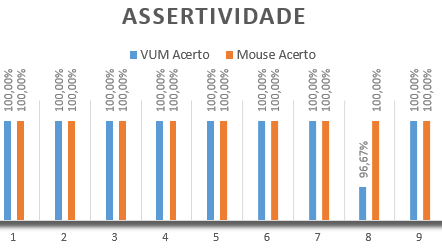
\includegraphics[scale=1]{img/assertividade.png}

\textbf{Fonte:} Autor.
\label{fig:assertividade}
\end{figure}

A Figura \ref{fig:tmc} apresenta o gráfico com os resultados do tempo médio de cada clique (TMC), em milissegundos. O TMC do \textit{mouse} comum foi de aproximadamente 6372,4 milissegundos. O VisiUMouse (VUM) teve o TMC de aproximadamente 16579,5 milissegundos.
\begin{figure}[htbp]
\caption{Resultados do teste comparativo.} 
\centering 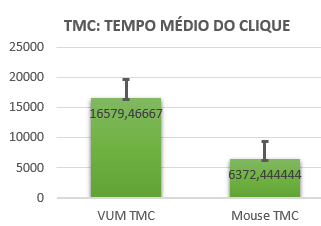
\includegraphics[scale=1]{img/tmc2.png}

\textbf{Fonte:} Autor.
\label{fig:tmc}
\end{figure}
















\begin{comment}
Exemplos do Template
\section{Motivação e objetivos}
\section{Contribuicoes}
\section{Producao cientifica}
\section{Organizacao da tese}
\noindent \textbf{Capitulo \ref{CAP2}}: descricao...
\noindent \textbf{Capitulo \ref{CAP3}}: descricaoo...
\noindent \textbf{Capitulo \ref{CAP4}}: descricao...
\noindent \textbf{Capitulo \ref{CAP5}}: descricao...

Exemplos do Template
\subsection{Exemplo de uma equação mais complexa}

  Equações mais complexas podem ser mais facilmente escritas com uso do programa TexAide. Como, por exemplo,

    \begin{equation}\label{Eq:sqrt_gamma_X}
    f_{\Gamma ^{{1 \mathord{\left/
    {\vphantom {1 2}} \right.
    \kern-\nulldelimiterspace} 2}} } (x;\alpha ,\lambda ) = \frac{{2\lambda ^\alpha  }}{{\Gamma (\alpha )}}x^{2\alpha  - 1} \exp \left( { - \lambda x^2 } \right).
    \end{equation}
    \[
    \alpha ,\lambda > 0.
    \]
    %
    em que $\Gamma(\cdot)$ é a função Gama. O programa TexAide é semelhante ao \textit{MathType} do Office, porém ao copiar e colar a equação em um arquivo tex, é gerado o código em LaTex referente a esta equação.

\section{Tabelas}

Tabelas são essenciais na apresentação de dados. A Tabela \ref{Tb:X_models} mostra um exemplo do uso deste tipo de elemento. Vale ressaltar que não é aconselhável o uso de linhas verticais em trabalhos acadêmicos e de pesquisa.

\begin{table}[h]
 \caption{Modelos estatísticos e suas relações.}%
 \label{Tb:X_models}
  \centering
\begin{tabular}{c c c c c}
 \hline
 &&&&\\
                                             &$\alpha ,\lambda  > 0$    &                               &$\alpha ,\lambda \rightarrow\infty$  &Homogêneo \\
                                             &$\gamma  \to 0$           & Heterogêneo                   &$\alpha / \lambda \rightarrow \beta$ & \\
                                             &$\mathop  \to \limits^D $ & $\sqrt\Gamma(\alpha,\lambda)$ &$\mathop  \to \limits^P $            &$\sqrt\beta$        \\
$\mathcal{N}^{-1/2}(x;\alpha,\gamma,\lambda)$& & & &\\
                                             &$\mathop  \to \limits^D $ & $\Gamma^{-1/2}(\alpha,\gamma)$&$\mathop  \to \limits^P $   &$\sqrt{\zeta^{-1}}$ \\
                                             &$\lambda \to 0$           &  Extremamente                 &$-\alpha / \gamma \rightarrow \zeta^{-1}$ & \\
                                             &$-\alpha ,\gamma   > 0$   &  Heterogêneo                  &$-\alpha ,\gamma \rightarrow\infty$ &Homogêneo \\
 &&&& \\
 \hline
 &&&&\\
                                             &$\alpha ,\lambda  > 0$    &                               &$\alpha ,\lambda \rightarrow\infty$  &Homogêneo \\
                                             &$\gamma  \to 0$           & Heterogêneo                   &$\alpha / \lambda \rightarrow \beta$ & \\
                                             &$\mathop  \to \limits^D $ &$\mathcal{K}_A(\alpha,\lambda,n)$&$\mathop  \to \limits^P $&$\sqrt\Gamma(n,n/\beta)$        \\
$\mathcal{G}_A(z;\alpha,\gamma,\lambda,n)$   & & & &\\
                                             &$\mathop  \to \limits^D $ & $\mathcal{G}_A^0(\alpha,\gamma,n)$&$\mathop  \to \limits^P $&$\sqrt\Gamma(n,n\zeta)$  \\
                                             &$\lambda \to 0$           &  Extremamente                 &$-\alpha / \gamma \rightarrow \zeta$ & \\
                                             &$-\alpha ,\gamma   > 0$   &  Heterogêneo                  &$-\alpha ,\gamma \rightarrow\infty$ &Homogêneo \\
&&&&   \\
 \hline

\end{tabular}
\end{table}


A Figura \ref{Fig:1} mostra o exemplo do uso do comando ``subfigure''. Apesar de aceitar diferentes tipos de imagens. É preferível que as imagens estejam no formato .eps. Isso garante que a imagem impressa seja exatamente aquela visualizada, como acontece com arquivos pdf.

\begin{figure}[!ht]
\centering
\subfloat[]{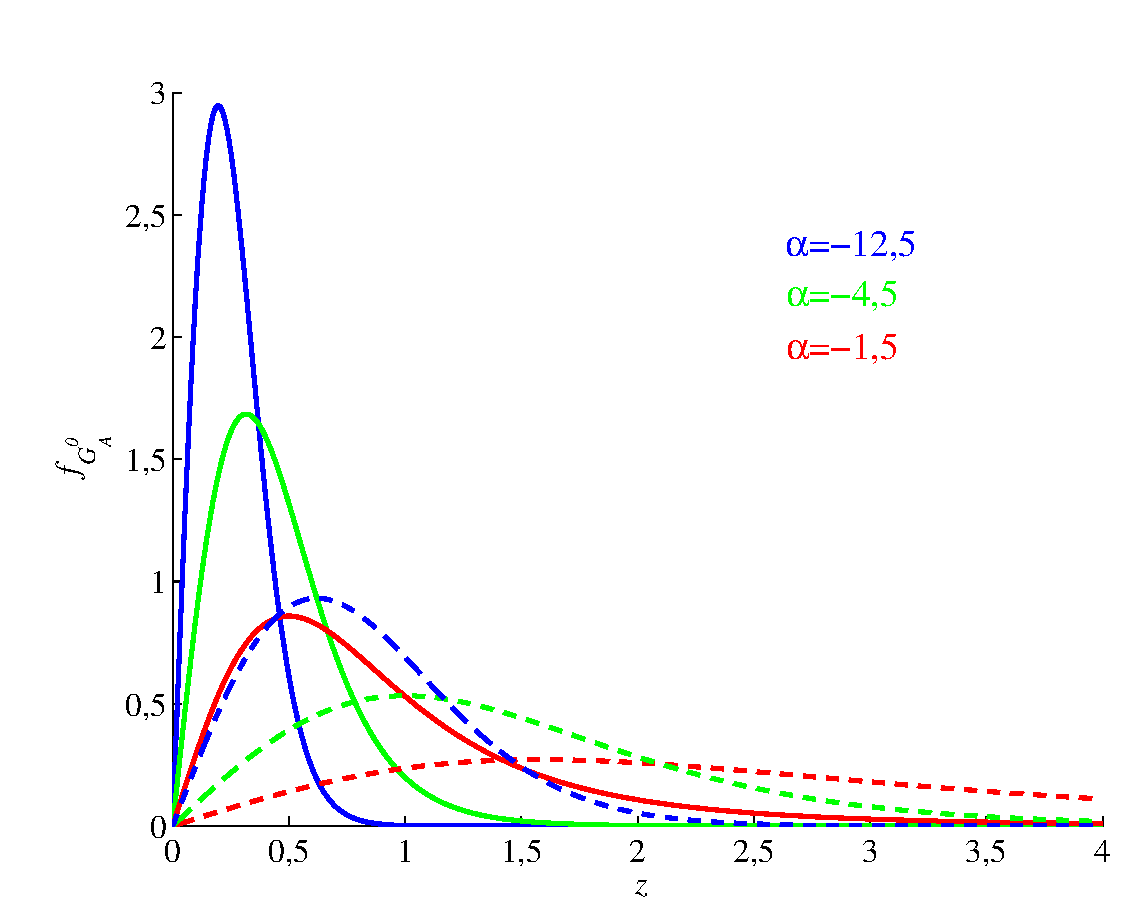
\includegraphics[scale=.65]{figures/fig1.eps}}\\
\subfloat[]{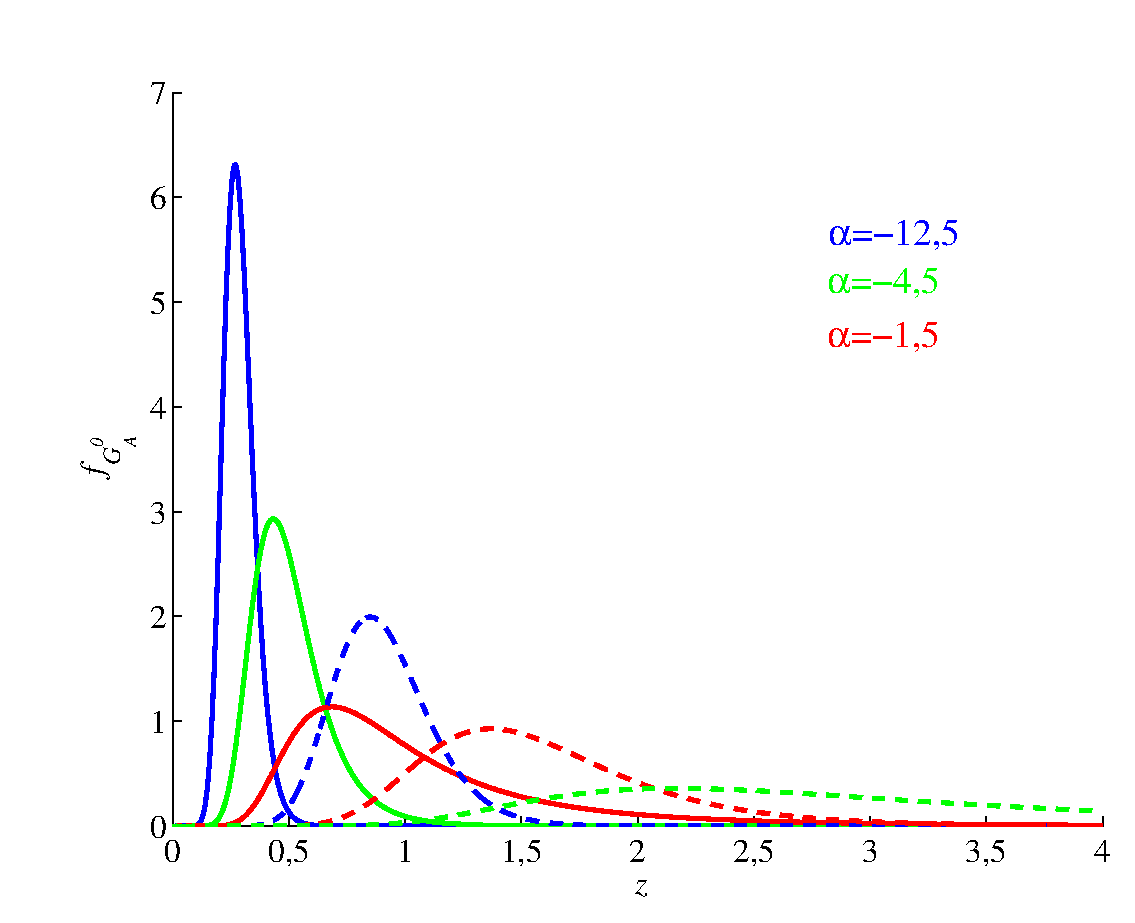
\includegraphics[scale=.65]{figures/fig2.eps}}
\caption{ Curvas de funções de probabilidade: (a) exemplo 1, (b) exemplo 2.} \label{Fig:1}
\end{figure}

\chapter{Método Proposto}\label{CAP3}
\chapter{Resultados Experimentais}\label{CAP4}
\chapter{Conclusão e Trabalhos Futuros}\label{CAP5}
\end{comment}